\documentclass{tufte-book}

\hypersetup{colorlinks}% uncomment this line if you prefer colored hyperlinks (e.g., for onscreen viewing)

%%
% Book metadata
\title{Hypercompression}
\author{Charles Holbrow}
%\publisher{Publisher of This Book}

%%
% If they're installed, use Bergamo and Chantilly from www.fontsite.com.
% They're clones of Bembo and Gill Sans, respectively.
%\IfFileExists{bergamo.sty}{\usepackage[osf]{bergamo}}{}% Bembo
%\IfFileExists{chantill.sty}{\usepackage{chantill}}{}% Gill Sans

%\usepackage{microtype}

%%
% Symbol for Euro Currency
\usepackage[official]{eurosym}

%%
% For nicely typeset tabular material
\usepackage{booktabs}

%%
% For graphics / images
\usepackage{graphicx}
\setkeys{Gin}{width=\linewidth,totalheight=\textheight,keepaspectratio}
\graphicspath{{graphics/}}

% The fancyvrb package lets us customize the formatting of verbatim
% environments.  We use a slightly smaller font.
\usepackage{fancyvrb}
\fvset{fontsize=\normalsize}

%%
% Prints a trailing space in a smart way.
\usepackage{xspace}

% Inserts a blank page
\newcommand{\blankpage}{\newpage\hbox{}\thispagestyle{empty}\newpage}

\usepackage{units}
% Control the formatting of lists
\usepackage{enumitem}

% Typesets the font size, leading, and measure in the form of 10/12x26 pc.
\newcommand{\measure}[3]{#1/#2$\times$\unit[#3]{pc}}

% Macros for typesetting the documentation
\newcommand{\hlred}[1]{\textcolor{Maroon}{#1}}% prints in red
\newcommand{\hangleft}[1]{\makebox[0pt][r]{#1}}
\newcommand{\hairsp}{\hspace{1pt}}% hair space
\newcommand{\hquad}{\hskip0.5em\relax}% half quad space
\newcommand{\TODO}[1]{\textcolor{red}{\bf TODO:#1}\xspace}
\newcommand{\ie}{\textit{i.\hairsp{}e.}\xspace}
\newcommand{\eg}{\textit{e.\hairsp{}g.}\xspace}
\newcommand{\na}{\quad--}% used in tables for N/A cells

 % This block sets up a command for printing an epigraph with 2
 % arguments - the quote and the author
\newcommand{\openFM}[3]{
\begin{fullwidth}
\rmfamily\huge

\noindent\allcaps{\textbf{#1}}\\ % The title
\rmfamily\LARGE
\noindent{#2} % The subtitle
\begin{spacing}{5}
\sffamily
\end{spacing}
\noindent{#3}
\end{fullwidth}
}

% This block sets up a command for printing an epigraph with 2
% arguments - the quote and the author
\newcommand{\openAFM}[3]{
\begin{fullwidth}
\rmfamily\huge

\noindent\allcaps{\textbf{#1}}\\ % The title
\rmfamily\LARGE
\noindent{#2} % The subtitle
\begin{spacing}{2.5}
\sffamily
\end{spacing}
\noindent{#3}
\end{fullwidth}
}

% Number parts and chapters
\setcounter{secnumdepth}{0}

% Title of my thesis project
\newcommand{\thesis}{Hypercompression\xspace}
\newcommand{\subtitle}{\TODO{Optional Subtitle}}
\newcommand{\polytempic}{Stochastic Tempo Transforms\xspace}
\newcommand{\refmod}{Reflection Modeler\xspace}

\begin{document}

% Front matter
\frontmatter
% Full title page
\openFM{\thesis}{\subtitle}{Charles Holbrow}

\noindent Bachelor of Music\\
\noindent University of Massachusetts Lowell, 2008\\

\vspace{30mm}

\begin{raggedright}
\noindent Submitted to the Program~in~Media~Arts~and~Sciences,\\
School~of~Architecture~and~Planning, in partial fulfillment\\
of the requirements for the degree of \textbf{Master~of~Science}\\
at the \textbf{Massachusetts~Institute~of~Technology} \\
\noindent August 2015\\
\noindent \textcircled{c}~2015~Massachusetts~Institute~of~Technology. All rights reserved. \\
\end{raggedright}

\begin{fullwidth}
\mbox{ }\\
\mbox{ }\\
\mbox{ }\\


\noindent Author: \hfill CHARLES HOLBROW\vspace{3pt}\hrule\vspace{6pt}
\flushright Program in Media Arts and Sciences\\
\flushright 7 August 2015 \\
\mbox{ }\\
\mbox{ }\\
\mbox{ }\\
 
\noindent Certified by: \hfill TOD MACHOVER\vspace{3pt}\hrule\vspace{6pt}
Professor of Music and Media\\
Program in Media Arts and Sciences\\
Thesis Supervisor\\
\mbox{ }\\ 
\mbox{ }\\

\noindent Accepted by: \hfill PATTIE MAES\vspace{3pt}\hrule\vspace{6pt}
Interim Academic Head\\
Program in Media Arts and Sciences\\

\thispagestyle{empty}  % Empty heads and feet - no page numbers.
\end{fullwidth}
 
%%% Local Variables:
%%% mode: latex
%%% TeX-master: "CharlesHolbrow_MAS_Thesis"
%%% End:


\chapter*{Abstract}
\label{ch:abstract}

\marginnote{\TODO{ Abstract is copy/pasted from another section, and
    is really just a placeholder}} While compression of mono and
stereo audio is well documented and understood,\cite{Giannoulis2012,
  Blesser1969} surround sound compression is relatively less explored.
\thesis expands on traditional audio compression model by adding
spatial control. This design introduces two additional high level
spatial parameters: \textbf{link angle} and \textbf{spread}. These
parameters extend the domain of the traditional compressor to include
surround sound spatial manipulation in addition to dynamics
processing, and unlock new creative possibilities for surround sound
designers.

%*******************************************************
% Readers
%*******************************************************

 \cleardoublepage
\openAFM{\thesis}{\subtitle}{Charles Holbrow}
\begin{fullwidth}
\mbox{ }\\
\mbox{ }\\
\mbox{ }\\ 
\vfill
\noindent The following person served as a reader for this thesis:\\
\vspace{10mm}

\noindent Thesis Reader: \hfill Joseph A. Paradiso\vspace{3pt}\hrule\vspace{6pt}
\flushright Associate Professor of Media Arts and Sciences\\
\flushright Program in Media Arts and Sciences\\
\flushright Massachusetts Institute of Technology\\

\thispagestyle{empty}  % Empty heads and feet - no page numbers.
\end{fullwidth}
 
\cleardoublepage 
\openAFM{\thesis}{\subtitle}{Charles Holbrow}
\begin{fullwidth}
\mbox{ }\\
\mbox{ }\\
\mbox{ }\\ 
\vfill
\noindent The following person served as a reader for this thesis:\\
\vspace{10mm}

\noindent Thesis Reader: \hfill James A. Moorer\vspace{3pt}\hrule\vspace{6pt}
\flushright Principal Scientist\\
\flushright Adobe Systems, Incorporated\\
\thispagestyle{empty}  % Empty heads and feet - no page numbers.
\end{fullwidth}
 

%%% Local Variables:
%%% mode: latex
%%% TeX-master: "CharlesHolbrow_MAS_Thesis"
%%% End:




\mainmatter
\tableofcontents
\cleardoublepage
\chapter{Introduction}
\label{ch:introduction}
\begin{fullwidth}
  \newthought{In the 6th century B.C.} Pythagoras discovered that
  dividing a resonating string into simple mathematical ratios
  produced harmonious musical intervals, while arbitrary ratios
  produced dissonance.  His observation is probably the first of the
  many explicit parallels between math and music that have been
  identified after his time. Today, we describe musical pitches, as
  integers within a given tuning system. We describe the tuning system
  with a mathematical formula that relates frequency to pitch. Musical
  time, rhythm and meter are commonly described numerically. Musical
  Transposition and inversion mirror mathematical functions, and
  borrow their names directly from mathematics.
\end{fullwidth}

As computers, amplifiers, and electronics become our primary tools for
creating manipulating, and performing music, mathematics and music
also become more interconnected. Nearly every modern musical
recording, broadcast, and stream is the summation of many digital
recordings that have been individually discretized, sampled
mathematically encoded, decoded, and digitally processed numerous
times before ever reaching our ears.\cite{Case2007} We might be
tempted to describe music today as applied mathematics, but doing so
betrays a fundamental quality of music: Musicality does not correspond
to mathematical elegance or precision. A musician will diverge from a
musical score to accomplish a particular artistic objective. A
vocalist does not abruptly change a pitch, but gently and carefully
lands on a pitch. A jazz musician might play slightly behind the
beat. A classical performer knows how to hold a fermata just long
enough. These intentional human artifacts are characterized more by a
feeling than by a formula.

The computer's inability to understand feeling has led to new genres
of music like EDM\sidenote[][-25mm]{EDM (Electronic Dance Music)
  features formulaic and repetitive grooves locked to a temporal grid,
  and often incorporates aggressive use of digital pitch correction,
  further exaggerating a robotic quality.}, Black
MIDI\sidenote[][-3mm]{Black MIDI is a musical genre that uses low
  fidelity audio samplers with a large number of MIDI notes over a
  short time. A single 3 minute Black MIDI track is likely to have
  over 100,000 MIDI notes. The name refers to the solid black
  appearance of the piano score.}, and Demoscene\sidenote{Demoscene
  music celebrates digital synthesis of compositionally complex
  electronic music and audio visualizations, using low level software
  interfaces, and including the design and programming of the music
  synthesizers as part of the composition.}, but these styles of music
feature (rather than fix) the inhuman nature of computers. If we want
to integrate a computer into the performance or production of truly
expressive music, we must capture perceived feelings formulaically,
and program the computer to reproduce them. This thesis describes
three different but related projects that confront this challenge from
contrasting perspectives: \refmod, \polytempic, and \thesis.

\section{\refmod}
\label{sec:refmod-intro}
\newthought {Music and space} are intimately connected. This project
explores how we can compose music using acoustic reflections in
architectural space as a medium. \refmod is a software tool that lets
us design and experiment with abstract acoustic lenses or ``sound
mirrors'' in 2 dimensions. It is directly inspired by the music and
architecture of Iannis Xenakis, a 20th century composer, music
theorist, architect and engineer. His collected works provide a guide
and perspective to all the projects in this thesis.

\section{\polytempic}
\label{sec:polytempic-intro}

\newthought{Music and Time} are inseparable. All music flows through
time, and depends on temporal constructs - the most common being meter
and tempo. Accelerating or decelerating tempo are common in many
styles of music, as are polyrhythms.  Music with multiple simultaneous
tempos or \textit{polytempic music} is less common, but still many
examples can be found. Few examples of music with simultaneous tempi
that shift relative to each other exist, and it is difficult for
musicians to accurately perform multiple tempi in parallel. Software
is an obvious choice for composing complex and challenging rhythms,
but modern compositional software makes this difficult. \polytempic
describes a strategy for composing music with multiple simultaneous
tempos that accelerate and decelerate relative to each other. In
\autoref{ch:polytempic} we derive an equation for smoothly ramping
tempi to converge and diverge as musical events within a score. We
show how this equation can be as a stochastic process to compose
previously inaccessible sonorities. 

\section{\thesis}
\label{sec:hypercompression-intro}
\newthought{We usually think of compression} in terms of
\emph{reduction}: We use data compression to reduce bit-rates and file
sizes, audio compression to reduce dynamic range. Record labels use
dynamic range compression as a weapon in the \emph{loudness
  war}\sidenote{``Loudness War'' is the popular name given to the
  trend of increasing percieved loudness in music recordings.
  Beginning in the 1990s, record labels have attempted to make their
  music louder than the competition, at the expense of audio
  fidelity}\cite{Deruty2014a}, resulting in some of today's music
recordings utilizing no more dynamic range than a 1909 Edison
cylinder.\cite{Katz2007}. A deeper study of dynamic range compression
reveals more subtle and artistic applications. A skilled audio
engineer applies compression to audio with the intention to improve
intelligibility, augment articulation, smooth a performance, shape
transients, extract ambience, de-ess vocals, balance multiple signals,
or even add distortion.\cite{Case2007} At its best, the compressor is
a tool for temporal shaping, rather than a tool for dynamic reduction.

\thesis expands the traditional model of a dynamic range compressor to
include spatial shaping. While unconventional, spatial
processing is a very natural fit for the compression paradigm. We can
think of sound as a medium that exists in time just as easily as we
can think of sound as something that exists in
space.\sidenote{Converting measurement of sound from the cycles per
  second (in the temporal domain) to wavelength (in the spatial
  domain) is common objective in acoustics and audio engineering
  practices. See \textit{The Sound Reinforcement Handbook} by G. Davis
  for examples.} The mathematics and implementation of the
Hypercompressor are described in detail in \autoref{ch:hypercompressor}.

\paragraph{Performance}
\thesis was used in the live performance of \textit{De
  L'Exp\'{e}rience}, a new musical work by composer Tod Machover for
Narrator, Organ, and Electronics. During the premier at the Maison
symphonique de Montr\'{e}al in Canada, \thesis was used to blend the
electronics with the organ and the acoustic space. In
\autoref{ch:hypercompressor} we also describe how Hypercompression fit
into this performance.

\section{Background}
\label{sec:background}
These projects build on the work and ideas of Iannis Xenakis, a 20th
century composer, architect, and engineer. Xenakis spent his youth
reading about astronomy, archeology, ancient literature, and
mathematics.\cite[]{Hoffmann2015} He studied music and engineering at
the Polytechnic Institute in Athens, Greece. By 1948, Xenakis had
graduated form the University, and moved to France where he began to
work for the french architect, Le Corbusier. The job put his
engineering skills to use, but he wanted to continute studying and
writing music.  While searching for a music mentor, he approached
Oliver Messiaen\sidenote{Messiaen was a prolific french composer
  known for rhythmic complexity. He was also regarded as an fantastic music
  teacher, and his students include Karlheinz Stockhausen, Pierre
  Boulez, and Quincy Jones.}, and asked if he should study harmony or
counterpoint. Messiaen later described his conversation with Xenakis:
\begin{quotation}``I think one should study harmony and
  counterpoint. But this was a man so much out of the ordinary that I
  said: No, you are almost 30, you have the good fortune of being
  Greek, of being an architect and having studied special
  mathematics. Take advantage of these things. Do them in your
  music.''\cite{Service2013}
\end{quotation}
Ultimately, Messiaen was rejecting Xenakis as a student, but we can
see how Xenakis did draw from disparate skills in his composition. The
score for his 1945 composition \textit{Metastasis}
(figure~\ref{fig:metastasis}), resembles an architectural blueprint as
much as it does a musical score.

\begin{figure*}[h]
  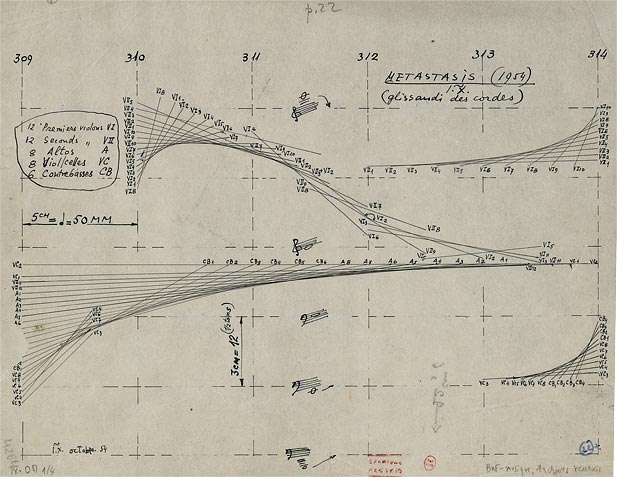
\includegraphics[width=\linewidth]{XenakisMetastasis.jpg}
  \caption{Excerpt from Iannis Xenakis' composition,
    \textit{Metastasis} (1954), measures 309-314. This score in this
    image was then transcribed to sheet music for the orchestral
    performance.}
  \label{fig:metastasis}
\end{figure*}

\subsection{The Philips Pavilion}
\label{sec:philips-pavilion-1}
\begin{figure}[h]
  \includegraphics[width=\linewidth]{PhilipsPavilion-TechnicalReview-01.pdf}
  \caption{The Philips Pavilion at the 1958 Brussels World Fair as
    shown in Volume 20 of the \textit{Philips Technical Review}, 1959}
  \label{fig:philips-pavilion-photo}
\end{figure}
In 1956, Le Corbusier was approached by Louis Kalff (Artistic Director
for the Philips corporation) and asked to build a pavilion for the
1958 World's Fair in Brussels. The pavilion was to showcase the sound
and lighting potential of Philips' technologies. Le Corbusier
immediately accepted, saying:
\begin{quotation}
  ``I will not make a pavilion for you but an Electronic Poem and a
  vessel containing the poem; light, color image, rhythm and sound
  joined together in an organic synthesis.''\cite{Lopez2011} 
\end{quotation}
The final product lived up to Le Corbusier's initial description. It
included:\cite{Lombardo2009}
\begin{enumerate}
\item A concrete pavilion, designed by architect and composer Iannis
  Xenakis
\item \textit{Interlude Sonoire} (later renamed \textit{Concret PH}), a
  tape music composition by Iannis Xenakis, approximately 2 minutes
  long, played between performances, while one audience left and
  pavillion, and the next audience another arrived.
\item A three channel, 8 minute tape music composition, by French-born
  composer Edgard Var\`{e}se
\item A system for spatialized audio across at least 350 loudspeakers
  distributed throughout the pavilion
\item An assortment of colored lighting effects, designed by Le Corbusier in
  collaboration with Philips art director Louis Kalff
\item Video consisting mostly of black and white still images,
  projected on two walls inside the pavilion
\item A system for synchronizing playback of audio and video,
  with the light effects and audio spatialization throughout the
  experience
\end{enumerate} 

\paragraph{The Role of Iannis Xenakis} During the initial design stage,
Le Corbusier determined that the shape of the pavilion building should
resemble a stomach, with the audience entering through one entrance,
and exiting through another. He completed initial sketches of the
pavilion layout, and then delegated the remainder of the design to
Xenakis.\cite{Clarke2012}

The architectural evolution of the pavilion from Le Corbusier's early
designs (figure~\ref{fig:le-corbusier-sketch}) through Xenakis'
iterations (figure~\ref{fig:xenakis-draw}), illustrates the impact
that Xenakis had on the project. An article in the \textit{Philips
  Technical Review}\cite{philips1958} gives a wonderfully detailed
account of Xenakis' process:
\begin{enumerate}
\item Xenakis was aware that parallel walls, or concave spherical
  walls would negatively impact audio perceptibility due to repeated
  or localized acoustic reflections.
\item To accommodate musical purpose of the space he decided to
  explore surfaces with varying curvature...
\item 
  \begin{marginfigure}
    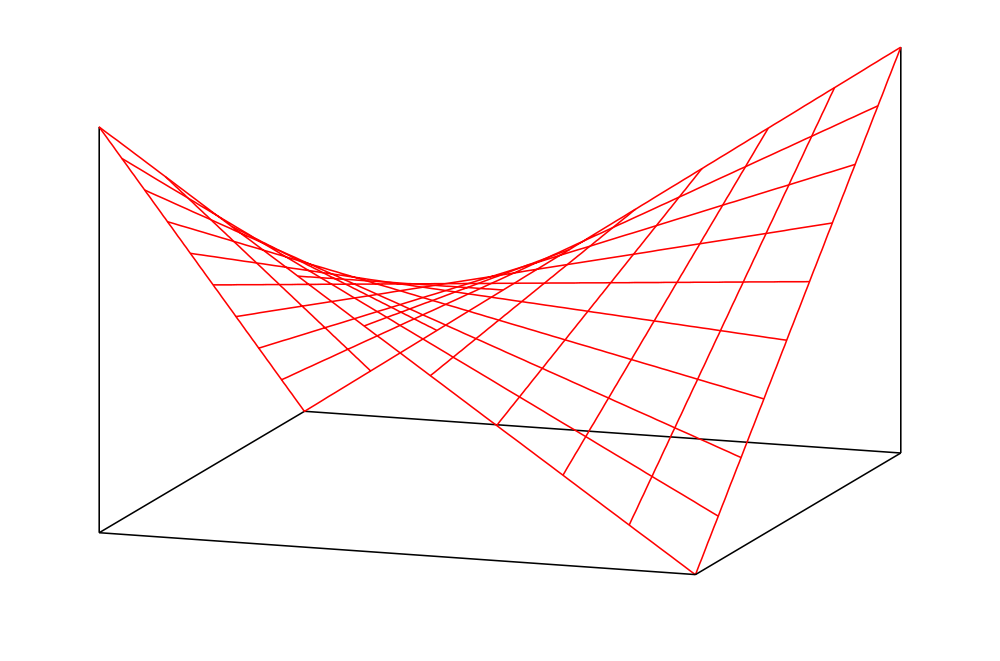
\includegraphics{hyperbolic-paraboloid}
    \caption{A ruled surface. For a surface to be considered ``ruled''
      every point on the surface must be on a straight line, and that
      line must lie on the surface. In Xenakis' time, ruled surfaces
      were useful in architecture, because they simplified the
      construction of curved surfaces by using straight beams.}
    \label{fig:ruled-surface}
  \end{marginfigure}...leading him to consider ruled surfaces such as
  the conoid and hyperbolic paraboloid. 
\end{enumerate}
We see Xenakis utilizing the drafting skills that he learned at the
Polytechnic Institute and continued to develop while working with Le
Corbusier. He also understood the mathematical formation of the ruled
surfaces that make up the structure. These surfaces even look familiar
from the Metastasis score (figure~\ref{fig:metastasis}). In his book
1963 book, \textit{Formalized Music}, Xenakis explicitly states that
the philips pavilion was inspired by his work on
\textit{Metastasis}.

\begin{figure*}[]
  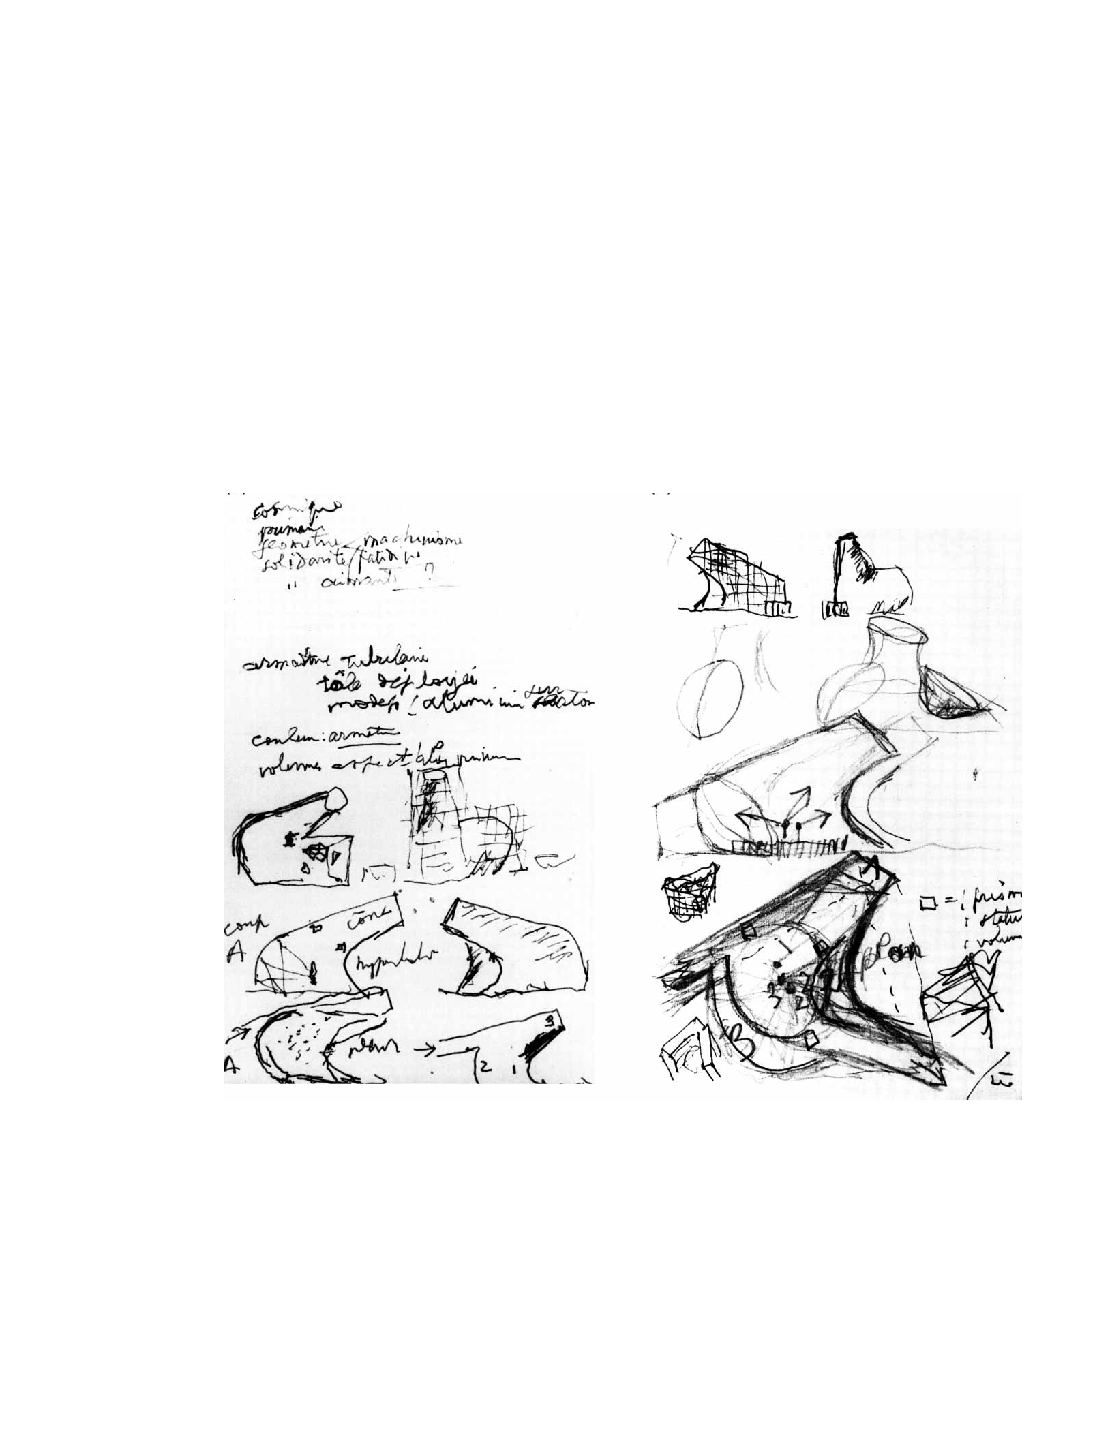
\includegraphics[width=\linewidth]{LeCorbusierDraw.pdf}
  \caption{Le Corbusier's design sketches for the Philips Pavilion,
    September \textendash{} October, 1956 (\textcircled{c} 2012
    Artists Rights Society, New York/ADAGP, Paris/FLC)}
  \label{fig:le-corbusier-sketch}
\end{figure*}

\begin{figure*}[h]
  % XenakisSketch.pdf or PhilipsDrawings.jpg
  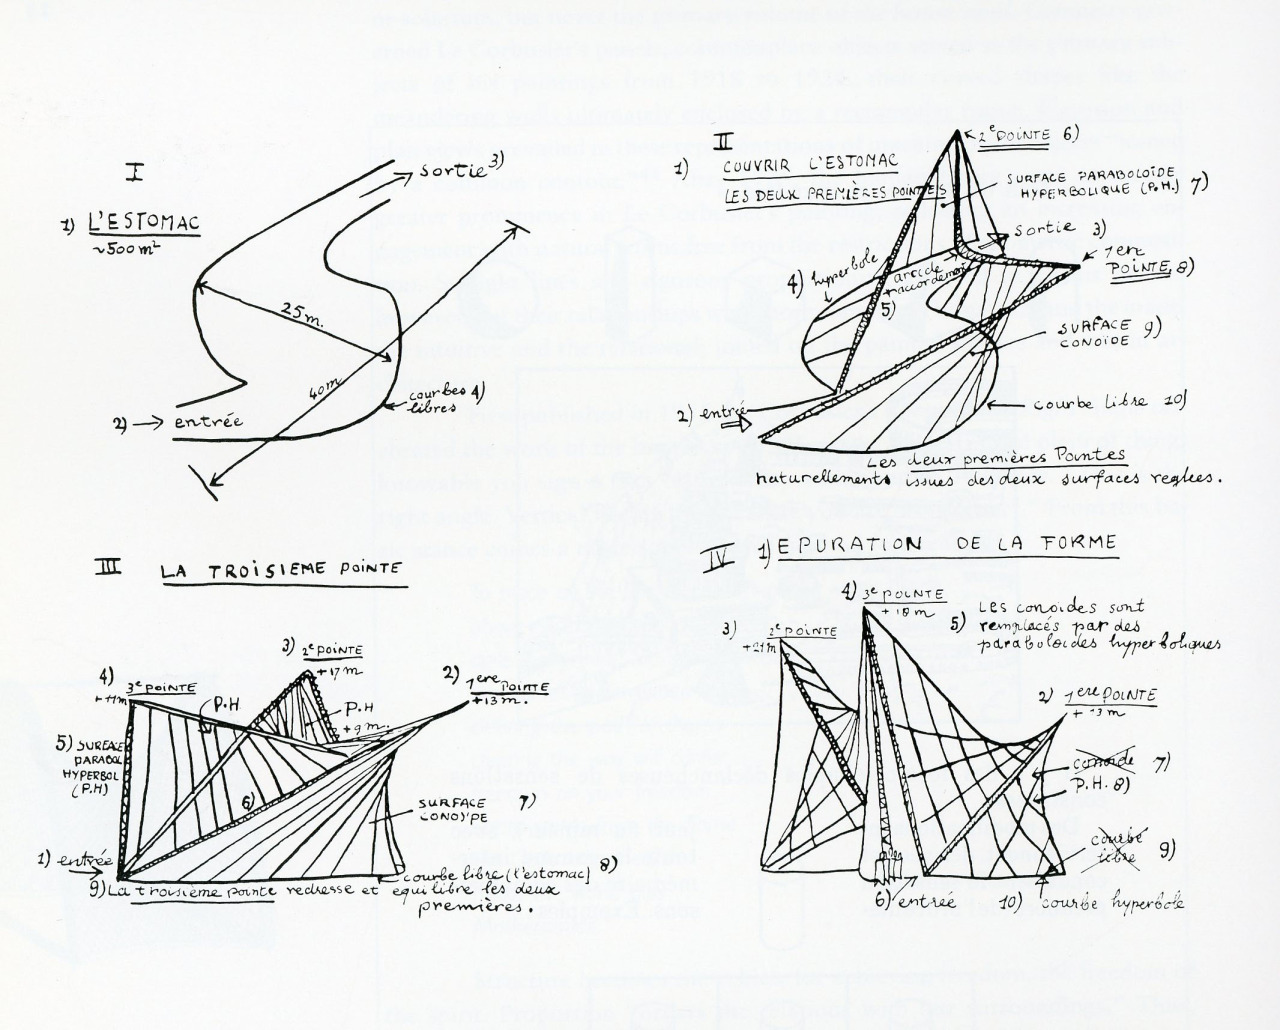
\includegraphics[]{PhilipsDrawings.jpg}
  \caption{Xenakis' early drawings of the Philips Pavilion as
    documented in volume 20 of the \textit{Philips Technical Review}.}
  \label{fig:xenakis-draw}
\end{figure*}

\section{Architecture and Music in Space and Time}
\label{sec:introduction-conclusion}

In \textit{Formalized Music},\cite{xenakis1992formalized} Xenakis
describes how developments in music theory mimic equivalent
developments in philosophy, mathematics, and the sciences. Plato, for
example, believed that all events transpire as determined by cause and
effect. While Plato and Aristotle both described causality in their
writing, it was not until the 17th century that controlled experiments
and mathematics corroborated the theory.\sidenote{In 1687, Isaac
  Newton published \textit{Philosophi\ae{} Naturalis Principia
    Mathematica} (\textit{Mathematical Principles of Natural
    Philosophy}), in which he compiled the 3 laws of motion that set
  the foundation for the study of \emph{classical mechanics}.}
Similarly, historical music follows deterministic progressions, and
music theory employs causal rules to describe counterpoint, tonality,
and harmonic movement.

Causality was largely used to describe physical phenomena until the
19th century when statistical theories in physics began to include
probabilistic notions.\sidenote{The Maxwell-Boltzmann distribution,
  which was first derived by James Clerk Maxwell in 1860, describes
  the probability distribution for the speed of a particle within an
  idealized gas. For more see
  \url{http://plato.stanford.edu/entries/statphys-statmech/}} Xenakis
noticed that more contemporary fields like \emph{probability theory}
and \emph{fuzzy logic} generalize and expand on the antecedent
theories of causality.

Xenakis thought that music composition should naturally follow
the progression that physics did, with the theory of music
generalizing and expanding on causal rules that had existed
previously. Indeed, starting in the late 19th century, and early 20th
century, composers like Strauss and Debussy began to bend the existing
rules of music theory, composing music that branched away from the
causal and tonal theories of the time. With the rise of
serialism\sidenote{Serialism is a technique for musical composition in
  which instances of musical elements (such as pitch, dynamics, or
  rhythm), are given numerical values. Sequences built from the values
  are ordered, repeated and manipulated throughout the composition.}
and indeterminate music\sidenote{In music, indeterminacy refers to the
  use of chance (such as rolling dice, or flipping coins) as part of
  the compositional process.}, composers such as Strauss, Debussy,
Stockhausen, Boulez, John Cage, Aaron Copland, and B\'{e}la Bart\'{o}k
began to use probability and chance in composition, the same way that
physicists were using probability to describe the material
world. However, to Xenakis' mathematical mind, serial music was no
less causal than the music it intended to supersede. He described
serial music as embodying ``virtually absolute
determinism.''\cite{xenakis1992formalized} Xenakis saw music theory as
a sub-set of mathematics and algebra. While musicians have a different
vocabulary, they also use mathematical principles to describe and
compose music. Because he understood mathematics as well as music, he
was able to identify how even in serialism and indeterminate music,
composers were only utilizing a small subset of algebraic theory. In
his own music, Xenakis wanted to generalize and expand the causal
framework that musicians and theorists had been using to compose and
understand music. This paralleled the developments in physics and
mathematics that helped him to form his opinions about music theory.
As a reference to \emph{chance} or \emph{stochos} Xenakis coined the
term \emph{stochastic music} to describe his development.

In \textit{Formalized Music}, Xenakis formally explains stochastic
music. It should be noted that some authors have interpreted his
description more explicitly. In \textit{Audible Design}, Trevor
Wishart, describes the stochastic process used to compose stochastic
music as:
\begin{quotation}
  ``A process in which the probabilities of proceeding from one state,
  or set of states. to another, is defined. The temporal evolution of
  the process is therefore governed by a kind of weighted
  randomness. which can be chosen to give anything from an entirely
  determined outcome, to an entirely unpredictable
  one.''\cite{Wishart1994}
\end{quotation}
It could be that the lack of a single clear definition by Xenakis is
the reason that few composers today identify as writing stochastic
music.

\paragraph{Xenakis' Reflection} In the Spring of 1976, Xenakis was
defending his doctoral thesis at the University of Paris. A
translation of his defense includes this statement:
\begin{quotation}
  ``The artist-conceptor will have to be knowledgeable and inventive
  in such varied domains as mathematics, logic, physics, chemistry,
  biology, genetics, paleontology (for the evolution of forms), the
  human sciences, and history; in short, a sort of
  \emph{universality}, but one based upon, guided by and oriented
  toward forms and architectures.'' \cite{russolo1986art}
\end{quotation}
From Xenakis' drawings we can deduce that he used the same tools,
skills, and philosophy to imagine and conceive both music and
space. His approach elevated both forms, and blurred the distinction
between the two. Maybe if we had kept using pen and paper to design
buildings and write music, the reality today would be closer to the
ideal that he imagined. Today, software for creating architecture or
composing music still favor corners to curves, and static pitches to
glissandi. More importantly, the software skills that we use to design
and manipulate space, and the skills that we use to compose music
mutually exclude each other.

This is where the projects described here make a contribution. As the
ideas that inspired Xenakis and other progressive 20th century
composers were taking root in contemporary music, the culture of
artistic form and composition was already beginning the transition
into the digital domain. However, there is no reason why digital tools
cannot favor stochastic procesees to linearity. There is no reason why
digital tools cannot treat music and architecture as equals. By
drawing from music, mathematics, computer science, acoustics, audio
engineering and mixing, sound reinforcement, multimedia production,
and live performance, we can create tools that allow us to
indiscriminately compose with space and sound.

\section{Universality}
\label{sec:universality}
At the MIT Media Lab, we celebrate the study and practice of projects
that exist outside of established academic disciplines. The Media Lab
(and the media) have described this approach as interdisciplinary,
cross-disciplinary, anti-disciplinary, or post-disciplinary;
emphasizing the clich\'{e} that traditional academics must become
experts in their field, and while narrowing their focus, they learn
\textit{more and more about less and less}, and eventually know
\textit{everything about nothing}.  \thesis is truly a Media Lab
project. It documents the creative process throughout the design,
development, and performance of a new type of audio signal
processor. In doing so, it draws from music, mathematics, computer
science, acoustics, audio engineering and mixing, sound reinforcement,
multimedia production, and live performance. How can we describe and
document a project with such broad subject material? Within a single
discipline, there is an accepted hierarchy of concepts, and we are
expected to develop a \emph{deep} understanding that penetrates this
hierarchy. We expect students to be literate in algebra, geometry and
calculus before studying physics. When we describe a physics problem,
we depend on an established collection of language, notation, and
theory.

This example reveals the curious tension between breadth and depth:
The \textit{depth} of a disciplinary approach provides the language
and abstraction that enable us to describe content and communicate at
a high level. Depth is essential for solving non-trivial
problems. However, solutions to the most complex and interesting
real-world projects always span multiple disciplines. It appears we
need breadth \emph{and} depth simultaneously.

One of the goals of this thesis is to bridge disciplines by describing
the material in a way that is accessible to readers that are not
experts in the all the fields involved. The work of Iannis Xenakis is
the perfect frame of reference because of it's powerful impact on
architecture, music, and culture.



\TODO{
The success of the Philips
Pavilion suggests the inherent value of the }


The challenge is to describe interdisciplinary projects so that it is
accessible to readers from all disciplines. This thesis proposes the
motivation for documenting media that exists outside of established
disciplines. It proposes a strategy for such documentation, and
employs this strategy by documenting the theory, implementation, and
application of \thesis.



%%% Local Variables:
%%% mode: latex
%%% TeX-master: "CharlesHolbrow_MAS_Thesis"
%%% End:


\chapter{Time Domain: \polytempic}
\label{ch:polytempic}
In \autoref{ch:introduction} (see figure~\ref{fig:metastasis}) we saw how
Xenakix was using ruled surfaces to create swarms of notes that move
together to create stochastic sonorities. The goal of \polytempic is
to enable composition with swarms of tempo modulations that move in
correlated, cohesive patterns. Music with two or more simultaneous
tempos (polytempic music) is itself not a new concept, and many
examples of polytemic music exist\cite{Greschak2003}. Slightly less
comon is polytempic music where continuous tempo accelerations or
decelerations are defined relative to each other.  This style of music
is well suited to tape music, because tape machines can play
recordings back at variable rates. However, it is difficult to control
the exact point (or phase) when de-synchronized tape becomes
re-aligned. Performative music with simultaneous tempi that accelerate
and decelearate realtive to each other is unusual, but does exist. In
a 1971 interview Composer Steve Reich described how he made the
transition to performative polytempic music after working on his tape
music composition, \textit{Come Out}:
\begin{quotation}
  ``1966 was a very depressing year. I began to feel like a mad
  scientist trapped in a lab: I had discovered the phasing process
  of Come Out and didn't want to turn my back on it, yet I didn't know
  how to do it live, and I was aching to do some instrumental
  music. The way out of the impasse came by just running a tape loop
  of a piano figure and playing the piano against it to see if in fact
  I could do it. I found that I could, not with the perfection of the
  tape recorder, but the imperfections seemed to me to be interesting
  and I sensed that they might be interesting to listen to.''\cite{Nyman2015}
\end{quotation}
Reich's experience illustrates what other composers and performers
have also encountered: It is quite difficult to perform polytempic
music accurately. In \textit{Piano Phase} Reich has two performers
playing the same 12 tone series on the piano. After a set number of
repetitions through the pattern, one performer begins to play slightly
faster until she is exactly one note ahead of the other performer, at
which point both performers play at the same rate for a time. This
process is repeated and iterated on, creating a live \emph{phasing}
effect without the pitch shifting that would occur when phasing analog
tape. If we compare a live performance\cite{Huisman1989} with a
programatic rendering\cite{Chen2014} of \textit{Piano Phase}, we can
hear how the programatic rendering is able to accelearate more
smoothly. The programatic example spends longer on the transitions
where the two parts are out of phase.

\section{Objective}
\label{sec:polytempic-objective}
Steve Reich composed \textit{Piano Phase} for two performers. In his
experimentation, he found that if the music is reasonably simple, two
performers can make synchronized tempo adjustments relative to each
other well enough to yield compelling results. To create stochastic
tempo transitions, our requirements are probably too demainding for
unassisted performers. Our goal is to compose and audition music
where:
\begin{enumerate}
  \item Swarms of an arbitrary number of simultaneous tempi
    coexist. 
  \item Each individual player within the swarm can continously
    accelerate or decelerate individually, but also as a member of a
    cohesive whole. 
  \item Each musical line can converge and diverge at explicit
    points. At each point of convergence the phase of the meter within
    the tempo can be set.
\end{enumerate}
We start by defining a single tempo transition. Consider the following
example shown in figure~\ref{fig:basic-tempo-change}:
\begin{itemize}
\item Assume we have 2 snare drum players. Both begin playing the same
  beat at 90 BPM in common time.
\item One performer gradually accelerates relative to the other. We want
  to define a continous tempo curve such that one drummer accelerates
  to 120 BPM.
\item So far, we can easily accomplish this with a simple linear tempo
  acceleration. However, we want the tempo transition to complete
  exactly when \emph{both} drummers are on a down-beat, so the the
  combined effect is a 3 over 4 rhythmic pattern.
\item We want the accelerating drummer to reach the new tempo after
  exactly 20 beats.
\item We also want the acceleration to complete in exactly 16 beats of
  the original tempo, so the drumer playing a constant tempo, and the
  the accelerating drummer are playing together.
\end{itemize}
\begin{figure*}[h]
  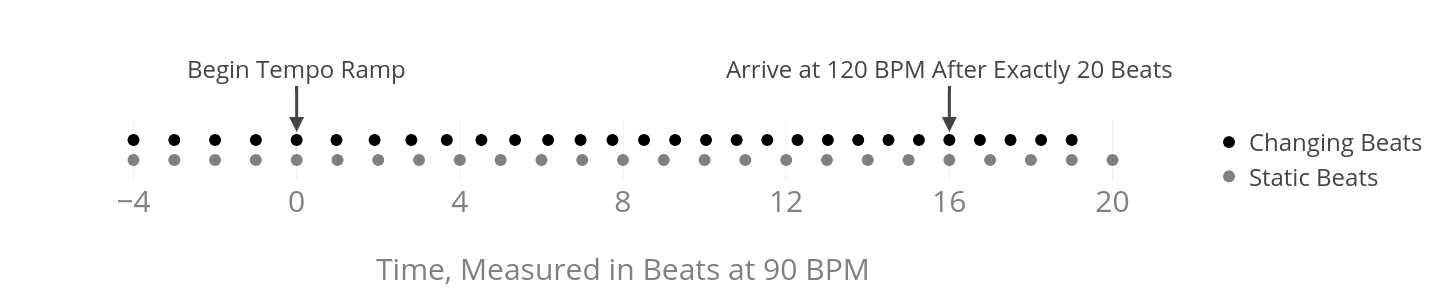
\includegraphics[width=\linewidth]{basic-tempo-transition.png}
  \caption[Tempo Transition]{Tempo Transition from 90 BPM
    to 120 BPM }
  \label{fig:basic-tempo-change}
\end{figure*}

\section{Solution}
\label{sec:polytempic-solution}
We are interested in both the number of beats elapsed in the static
tempo \emph{and} in the changing tempo, and the absolute tempo. Let us
think of the number of beats elapsed as our \emph{position}, and the
tempo as our \emph{rate}, we see how this resembles a physics
problem. If we have a function that describes our tempo (or rate), we
can integrate that function, and the result will tell us our number of
beats elapsed (or position). Given the above considerations, we define
our tempo curve in terms of 5 constants:
\\[5mm]
\begin{fullwidth}
\begin{itemize}
  \item Time $t_0=0$, when the tempo transition begins
  \item A known time, $t_1$, when the tempo transition ends
  \item A known starting tempo, $\dot{x}_0$
  \item A known finishing tempo, $\dot{x}_1$
  \item The number of beats elapsed in the changing tempo between
    $t_0$ and $t_1$, $x_1$
\end{itemize}
\end{fullwidth}
The tension of the tempo curve determines how many beats elapse during
the transition period. The curve is well-defined for some starting
acceleration $a_0$ and finishing acceleration $a_1$, so we define the
curve in terms of linear acceleration. Using Newtonian notation we can
describe our tempo acceleration as:
\begin{equation}
	\label{accel}
    \ddot{x}_1 = a_0 + a_1t_1
\end{equation}
Integrating linear acceleration (\ref{accel}) yields a quadratic
velocity curve. The velocity curve describes the tempo (in beats per
minute)\marginnote{We must specify the same time units for input
  variables like $t_1$ and $\dot{x_1}$. I prefer \textit{minutes} for
  $t_1$ and \textit{beats per minute} for $\dot{x_1}$ over
  \textit{seconds} and \textit{beats per second}} with respect to
time.
\begin{equation}
	\label{bpm}
    \dot{x}_1 = \dot{x}_0 + a_0t_1 + \frac{a_1t_1^2}{2}
\end{equation}
Integrating velocity (\ref{bpm}) gives us a function describing the number 
of beats elapsed with respect to time.
\begin{equation}
	\label{beats-elapsed}
	x_1 = x_0 + \dot{x}_0t_1 + \frac{a_0t_1^2}{2} + \frac{a_1t_1^3}{6}
\end{equation}
With equations (\ref{bpm}) and (\ref{beats-elapsed}), we can solve for our 
two unknowns, $a_0$ and $a_1$. First we solve both equations for $a_1$:
\begin{displaymath}
    \label{a1-solution}
    a_1=
    \frac{-2}{t_1^2}(\dot{x}_0-\dot{x}_1 + a_0t_1)=
    \frac{-6}{t_1^3}(\dot{x}_0-x_1 + \frac{a_0t_1^2}{2})
\end{displaymath}
Assuming $t_1 \neq 0$, we solve this system of equations for $a_0$:
\begin{equation}
	\label{a0-result}
	a_0=\frac{6x_1-2t_1(\dot{x}_1+2\dot{x}_0)}{t_1^2}
\end{equation}
Evaluating (\ref{a0-result}) with our constants gives us our starting
acceleration. Once we have $a_0$ we can solve (\ref{bpm}) for $a_1$, and 
evaluate (\ref{bpm}) with $a_1$ and $a_0$ to describe our changing tempo 
with respect to time.

\section{Implementation}
\label{sec:polytempic-implementation}

Bryn Bliska Tide

\begin{figure*}[h]
  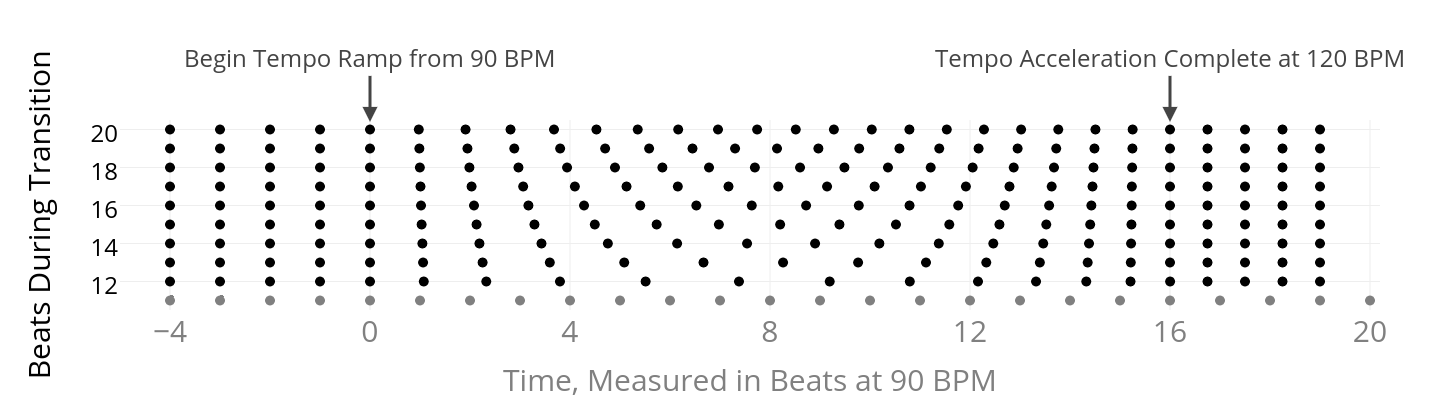
\includegraphics[width=\linewidth]{stochastic-tempi.png}
  \caption{Stochastic Tempo Transition from 90bpm to 120bpm}
  \label{fig:metastasis}
\end{figure*}


\section{Polytempic Music and Polymetric Music}
\label{sec:polytempic-vs-polymetric}
It is easy to confuse poly tempic music with polymetric music.  Pieces
where multiple meter
Other notable composers
of the time include John Cage, who wrote wrote what he called, Chance
Music, and Stockhausen, Boulez and Berio who wrote aleatoric music.



Eliot Carter: Polymetric Modulation. 
Steve Reich: Piano Phase
Paper: realtime representation of 
Paper: Stochos: Software for Real-Time Synthesis of Stochastic Music

John Cage: Chance Music
Karlheinz Stockhausen, Pierre Boulez, Luciano Berio: Aleatoric music

\section{Contribution}
\label{sec:polytempic-contribution}

and finishes the tempo transition slightly different tempos.

To audition stochastic tempo transitions, we can create software tools
that promt musicians with visual cues or aural cues, 
More flexible Digital Audio Workstations (DAWs) like Reaper and
Digital Performer include workarounds for auditioning simultaneous
tempo. 

For example we 

Xenakis was among a group of
20th century composers who were searching for ways to push the
boundaries of established music composition.


%%% Local Variables:
%%% mode: latex
%%% TeX-master: "CharlesHolbrow_MAS_Thesis"
%%% End:

\chapter{The Hypercompressor}
\label{ch:hypercompressor}

The motivation for Hypercompression came during the development of
Vocal Vibrations, an interactive music installation about the human
voice and about engaging the public in singing.\cite{Holbrow2014} The
project featured a Music Concr\`{e}te composition, \textit{The Chapel}
by Tod Machover, which was mixed in a 10 channel surround sound
format and played throughout the installation. During the mixing
process, I noticed an important surround sound tool missing from my
mixing workflow. When mixing in mono or stereo, audio
compression\marginnote{Unless noted otherwise, ``compression'' is used
  in this thesis to describe dynamic range compression, as opposed to
  data compression.} lets us meticulously shape and balance sounds in
time. I found myself wishing I could shape and position sounds in
space just as easily.

\section{Building on the Compression Paradigm}
The design, implementation, and use of traditional dynamic range
compression is well documented in the
literature,\cite[]{Giannoulis2012,Case2007,Deruty2014} so we will
describe dynamic range compression only as much as is needed to
explain the foundation for \thesis. Imagine we are mixing a vocal pop
performance, and during the verse our vocalist is singing moderately
loud, or \textit{mezzo-forte}. At the beginning of the chorus, our
singer wants a full and powerful sound, so she adjusts the dynamic to
very loud, or \textit{fortissimo}. However, the new louder dynamic
interrupts the balance between the vocals and the other instruments in
our mix. We like the powerful sound of our singer's
\textit{fortissimo} performance, but our balance would be improved if
we had the volume of a \textit{forte} performance instead. One option
is to manually turn down the vocalist during the chorus, which in some
cases this is the best solution. When we want more precise control, we
can use a compressor.

\subsection{Traditional Compression}
\label{sec:trad-compr}
A compressor is essentially an automated dynamic volume control.  Most
compressors include at least four basic parameters in the user
interface that allow us to customize its behavior: \textit{threshold},
\textit{ratio}, \textit{attack time}, and \textit{release time}.  We
can send our vocalist's audio signal through a compressor, and
whenever her voice exceeds the gain level set by our threshold
parameter, the signal is automatically attenuated. As the input signal
further exceeds the threshold level, the output is further attenuated
relative to the input signal. The ratio parameter determines the
relationship between the input level and output level as shown in
figure~\ref{fig:comp-ratio}.

\begin{marginfigure}
  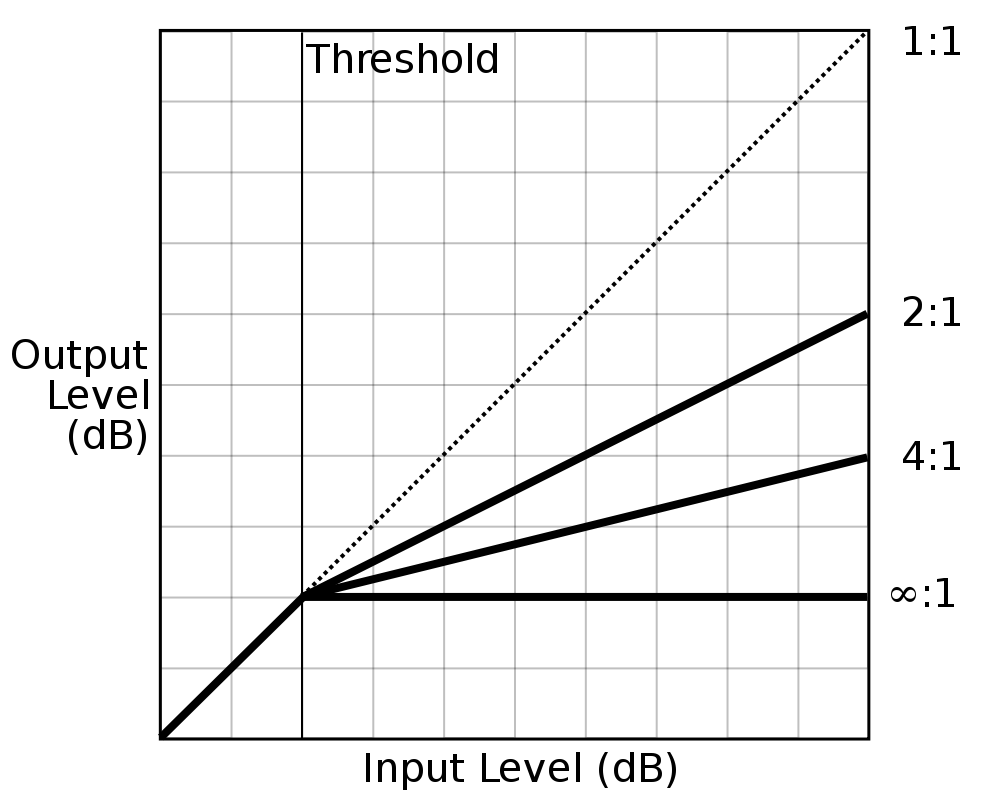
\includegraphics[]{CompressionRatio.png}
  \caption{``Compression ratio'' by Iain Fergusson. Licensed under
     Public Domain via Wikimedia Commons 
     \url{https://commons.wikimedia.org/wiki/File:Compression_ratio.svg\#/media/File:Compression_ratio.svg}
   }
  \label{fig:comp-ratio}
\end{marginfigure}

Threshold and ratio settings are essential for controlling dynamic
range, but the power and creative flexibility of the compressor comes
with the attack time and release time parameters. These parameters
determine the speed at which the compressor attenuates (attack time)
and disengages (release time) when the input signal exceeds the
threshold. By adjusting the attack and release times, we can change
the temporal focus of the compressor.
\begin{itemize}
\item Perhaps we want the compressor to engage or disengage at the
  time scale of a musical phrase. We could set our attack time long
  enough to let transients through without engaging the compressor
  significantly (try 20 milliseconds). If our release time is quite
  long (try 300 milliseconds), and we set our threshold and ratio
  carefully, we might be able to convince the compressor to smooth
  musical phrases.
\item If we want our compressor to focus on syllables instead of
  phrases, we can shorten our attack and release times (try 10
  milliseconds and 40 milliseconds respectively). When the compressor
  engages and disengages at each syllable, it imparts a different
  quality (sometimes described as ``punch'').
\item If we reduce our attack and release parameters enough, we can
  instruct our compressor to engage and disengage at the time scale of
  an audio waveform, compressing individual cycles. This will distort
  an audio signal, adding odd order harmonics,\sidenote{Not every
    compressor model can react quickly enough to distort a
    waveform. The Dbx 160 and Teletronix LA2A are known to be fast
    enough to distort.} and imparting an entirely different quality.
\end{itemize}
The attack and release times listed here are a rough guide only.  The
exact function of these parameters varies from one model of compressor
to another, and results also depend on the audio input material and
on the threshold and ratio settings. The results of audio
compression can sometimes be characterized better by a feeling than a
formula.

\begin{figure*}
  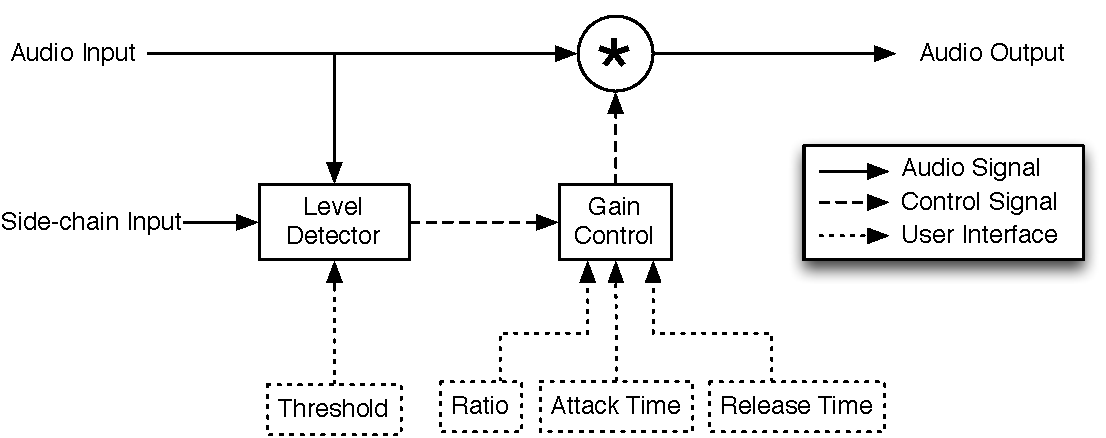
\includegraphics[width=\linewidth]{hypercomp/SimpleCompressor.pdf}
  \caption{Block diagram of a simple traditional dynamic range
    compressor.}
  \label{fig:comp-block}
\end{figure*}

\subsection{Side-Chain Compression}
\label{sec:side-chain-compr}
Compressors often have an additional operational mode that is the
primary inspiration for Hypercompression. We know that compressors
automatically reduce the gain of a signal that exceeds a given
threshold. Some compressors allow us to attenuate the level of a
signal when a \emph{different} signal exceeds the threshold
level. Models that suports side-chain compression have a second audio
input. When we switch the compressor into side-chain mode, the
compressor attenuates the first signal only when the second signal
exceeds the threshold.

Side-chain compression is often used to moderate the balance of kick
drum and bass guitar. If the bass guitar is briefly attenuated just
enough just the right amount each time the kick drum hits, we can set
the kick and bass guitar at exactly the gain levels we want without
one masking the other. Because the bass guitar is only briefly
attenuated, it will not be perceived as any quieter.

In this example we use the kick drum to create a gain envelope for our
bass guitar. The kick \emph{pushes} the bass to make room for
itself. The attack time and release time parameters give control over
this behavior in the temporal domain. The next step is to
expand this model to add control in the spatial domain.

\section{Ambisonics}
\label{sec:ambisonics}
Ambisonics is a technique for encoding and decoding three-dimensional
surround sound audio.\cite[-15mm]{Gerzon1973,Gerzon1985} Ambisonic
audio differs from other surround sound formats like $5.1$ and $7.1$
in that it does not depend on a particular speaker configuration. An
ambisonic recording can be decoded on any surround sound speaker
configuration without disarranging the spatial contents of the audio
recording.

Imagine we use an omnidirectional microphone to record an acoustic
instrument at a sample rate of 44.1 kHz. We sample and record 44100
samples every second that represent the air pressure at the microphone
capsule during the recording. Our omni-directional microphone is
designed to treat sound arriving from all angles equally. The
omnidirectional microphone sums together sounds arriving from all
angles and the acoustic directional information is lost.

If we want to encode, decode, transmit, or play audio that preserves
full sphere 360 degree information, ambisonics offers a solution.
Ambisonic audio uses \textit{spherical harmonics} to encode surround
sound audio that preserves the direction-of-arrival information that
discrete channel recordings (such as mono and stereo) cannot fully
capture.

\subsection{Spherical Harmonics}
\label{sec:spherical-harmonics}
We know that we can construct any monophonic audio waveform by summing
a (possibly infinite) number of harmonic sine waves (Fourier
series).\sidenote{An excellent description of the transformation between
  the time domain and frequency domain can be found at
  \url{http://betterexplained.com/articles/an-interactive-guide-to-the-fourier-transform/}}
For example, by summing odd \textit{order} sine harmonics at a given
frequency $f$, $(1f, 3f, 5f, 7f, \ldots )$, we generate a square wave
with fundamental frequency $f$. As the order increases, so does the
temporal resolution of our square wave.

By summing sinusoidal harmonics, we can generate any continuous
waveform defined in two dimensions (one input parameter and one
output). Similarly, by summing \emph{spherical harmonics}, we can
generate any continuous shape defined over the surface of a
three-dimensional sphere (two input parameters, or polar angles, one
output). Where a traditional monophonic audio encoding might save one
sample 44100 times per second, an ambisonic encoding would save one
sample \emph{for each spherical harmonic} 44100 times per second. This
way we capture a three-dimensional sound image at each audio sample.
The number of spherical harmonics we encode is determined by our
\textit{ambisonic order}. As our ambisonic order increases, so does
the angular resolution of our result on the surface of the sphere.

\subsection{Spherical Harmonic Definition}
For encoding and decoding ambisonics, the convention is to use the
real portion of spherical harmonics as defined in
equation~\ref{eq:spherical}, where:
\begin{itemize}
\item $Y_{n}^{m}(\varphi,\vartheta)$ is a spherical harmonic that
is:\marginnote{Some literature on spherical harmonics swaps the names
  of \textit{order} and \textit{degree}. In this thesis we use
  $Y_{order}^{degree}$. In literature where $Y_{degree}^{order}$ is
  used, the function of the subscript and superscript remain
  unchanged; only the names are inconsistent.}
\begin{itemize}
\item of order, $n$
\item of degree, $m$
\item defined over polar angles $(\varphi, \vartheta)$
\end{itemize}
\item $N_n^{|m|}$ is a normalization factor.\sidenote{In ambisonic
    literature (and software), there are multiple incompatible
    conventions for the normalization of spherical harmonics. The
    Hypercompressor uses the \textit{Furse-Malham} (FuMa)
    normalization convention.}
\item $P_n^{|m|}$ is the associated Legendre function of order $n$
  and degree $m$.
\end{itemize}
\begin{equation}
Y_{n}^{m}(\varphi,\vartheta)=N_n^{|m|}P_n^{|m|}(\sin{\vartheta})
\begin{cases}\label{eq:spherical}
\sin{|m|\varphi},&  \text{for $m<0$}\\  
\cos{|m|\varphi},& \text{for $m\geq 0$}\\
\end{cases}
\end{equation}
Given equation~\ref{eq:spherical}, we can define an ambisonic
audio recording as:
\begin{equation}
f(\varphi,\vartheta,t)=\sum\limits_{n=0}^N\sum\limits_{m=-n}^nY_n^m(\varphi,\vartheta)\phi_{nm}(t)
\label{eq:ambisonics}
\end{equation}
Where:
\begin{itemize}
\item $\varphi$ and $\vartheta$ describe the polar angle of sound
  arrival in two dimensions.\sidenote{Note that ambisonics uses polar
    angles to describe the angle of arrival of sound. These are
    similar to spherical coordinates, minus the inclusion of
    \textit{radial distance}. Distance is not part of the ambisonic
    specification.}
\item $t$ is time
\item $\phi_{nm}(t)$ are our \textit{expansion coefficients}, described
  below.
\end{itemize}
\begin{figure}[h]
  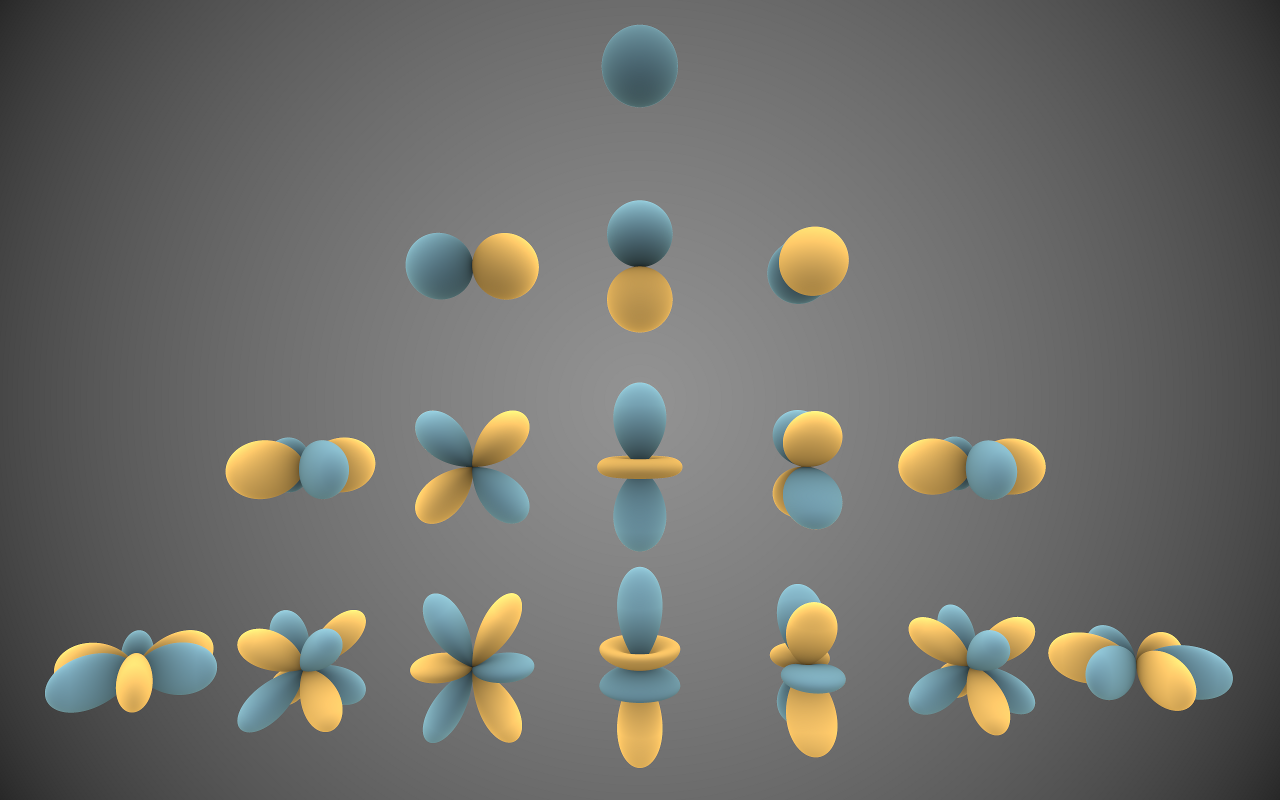
\includegraphics[width=\linewidth]{SphericalHarmonics.png}
  \caption{Spherical harmonics $0$th order (top row) through $3$rd
    order (bottom row). This for image shows the output of
    $Y_{n}^{m}(\varphi,\vartheta)$ for $n=0,n=1,n=2,$and $n=3$. The
    distance of the surface from the origin shows the value at that
    angle. Darker blue regions are positive, while lighter yellow
    regions are negative. Image credit: Ingo Quilez, licensed under
    \textit{Creative Commons Attribution-Share Alike 3.0 Unported}.}
  \label{fig:spherical-harmonics}
\end{figure}

\subsection{Spherical Harmonic Expansion Coefficients}
\label{sec:spher-harm-expans}
In our monophonic recording example, we save just one digital sample
44100 times per second, with each saved value representing the air
pressure at a point in time. We know that by summing the correct
combination of spherical harmonics, we can describe any continuous
function over the surface of a sphere. Instead of sampling air
pressure directly, we sample a coefficient describing the weighting of
each spherical harmonic 44100 times per second. The resulting sphere
encodes the pressure including the direction of arrival
information. The weighting coefficients or \textit{expansion
  coefficients} are recorded in our audio file instead of values
representing air pressure directly. Now, by summing together our
weighted spherical harmonics, we can reconstruct the fluctuations in
pressure including the angle of arrival information. We can recall
this snapshot of information at our 44.1 kHz audio sample rate.

\subsection{Ambisonic Encoding}
\label{sec:usage}
There are two ways to create an ambisonic recording. First, we can use
a soundfield microphone to record an acoustic soundfield. Soundfield
microphones like the one developed by Calrec Audio can capture angle
of arrival information with the spatial resolution of first order
ambisonics.\cite[-1in]{Ferrar1979} Alternatively, we can algorithmically
encode pre-recorded sources, creating virtual sources in an
ambisonic bus.\cite[-0.4in]{Malham1995}

\section{Ambisonic Conventions used for Hypercompression}
\label{sec:ambis-conv-used}
This thesis follows ambisonic convention for describing axis of
rotation. The x-axis points forward, the y-axis point left, and the
z-axis points up. Polar angles are used to describe orientation with
$0\degree$ azimuth being forward, and increasing as we move to the
left. $0\degree$ elevation also points forward, and increases as we
move upward, with $90\degree$ being strait up along the z-axis. When
working with ambisonics, multiple inconpatible conventions exist for
ordering and normalizing spherical harmonics.\cite{Nachbar2011} The
Hypercompressor uses \textit{Furse-Malham} normaliation
(FuMa)\cite{Malham2003}, and first order ambionics with
\textit{B-format}\cite{Hollerweger2008} channel ordering. B-format
ordering labels the four first-order ambisonic channels as W, X, Y,
and Z, with W being the spherical harmonic of order zero and degree zero,
and X, Y, and Z being the ressure gradient components along their
respective axes. 

\section{Hypercompressor Design}
\label{sec:hypercomp-design}
\begin{figure*}
  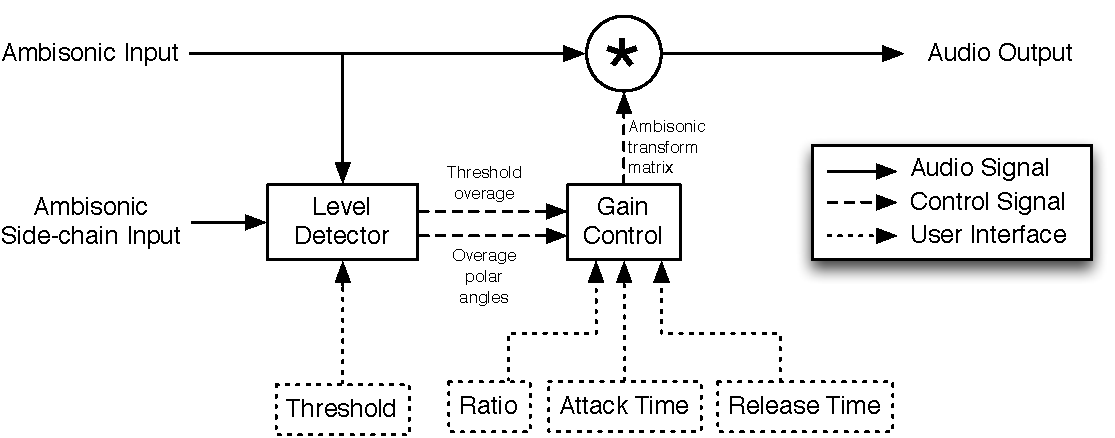
\includegraphics[width=\linewidth]{hypercomp/AmbisonicCompressor.pdf}
  \caption{Block diagram of the Hypercompressor.}
  \label{fig:hypercomp-block}
\end{figure*}
\noindent The Hypercompressor (or ambisonic compressor) combines the traditional
model of compression with the surround sound capability of
ambisonics. Given ambisonic input, and an optional ambisonic
side-chain input, the ambisonic compressor is intended to process our
input material in one of two modes:
\begin{enumerate}
\item Standard mode: We set a compression threshold, similar to on a
  traditional compressor. When a region in our surround sound input
  material exceeds the set threshold, the compressor engages and
  attenuates only that region.
\item Side-chain mode: This mode takes advantage of a second ambisonic
  input to our signal processor. When the gain of spatial region in
  our secondary input exceeds our threshold, we attenuate that same
  region in the the main input, and output the results.
\end{enumerate}
In both modes, our ambisonic compressor must attenuate and release
attenuation according to the attack time and release time
parameters. The block diagram for our new hypercompressor
(figure~\ref{fig:hypercomp-block}) can remain largely unchanged from
the the block diagram for our traditional compressor in
figure~\ref{fig:comp-block}. The most important changes are:
\begin{itemize}
\item Our audio signals must be updated to handle encoded
  ambisonics. This is as simple as increasing the number of channels
  on each solid black connection in figure~\ref{fig:comp-block}. The
  hypercompressor works with first order ambisonics, so every audio
  path must carry four audio channels.
\item On a traditional compressor, the level detector only needs to
  detect the difference between the gain of the input signal and the
  gain specified by the threshold parameter. Our ambisonic level detector
  needs to decode the incoming signals and identify both a threshold
  overage and the region where the overage occurred.
\item Our gain control module needs to listen to the input coming from
  the level detector module and be able to attenuate the specific
  regions that exceed our threshold parameter.
\end{itemize}

\subsection{Level Detection Module}
\label{sec:an-accurate-level}
In \textit{Spatial Transformations for the Alteration of Ambisonic
  Recordings}, Matthias Kronlachner describes
one approach for making a visual ambisonic level meter:\cite{Kronlachner2014} 
\begin{enumerate}
\item Choose a series of discrete points distributed on the surface of
  a sphere. Ideally the points are equally distributed, so the
  vertices of platonic solid shapes like the dodecahedron (12-sided
  polyhedron) and icosahedron (20-sided polyhedron,
  figure~\ref{fig:icosahedron}) work well. For spatial accuracy,
  Kronlachner recommends a spherical $t$-design with 240 points
  described by Hardin and Sloane.\cite{Hardin1996}
\item Evaluate each spherical harmonic at every point chosen. Cache
  the results in a matrix. 
\item With the cached spherical harmonics, it is then possible to
  calculate the RMS and peak values more efficiently at the audio
  rate.
\item A level meter does not need to refresh the display at the audio
  sample rate, so it is acceptable to interpolate between the points
  on the sphere and update the graphical representation at the
  control rate, which could be as slow as 30 Hz (approximately every
  33 milliseconds).
\end{enumerate}
\begin{marginfigure}
  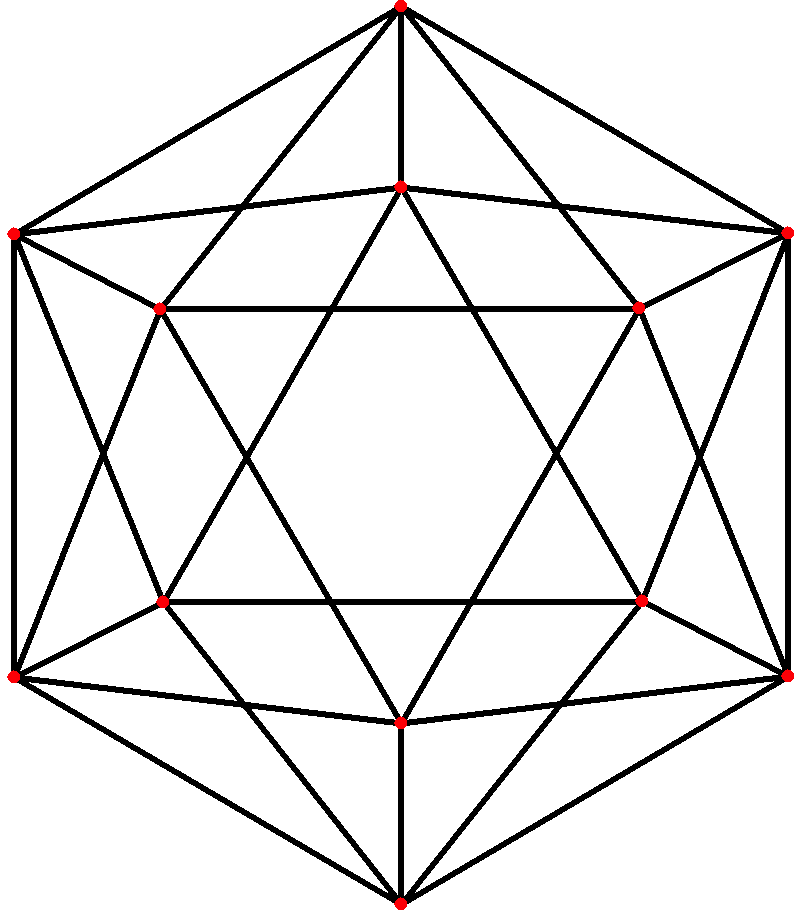
\includegraphics{hypercomp/Icosahedron.png}
  \caption{An icosahedron.}
  \label{fig:icosahedron}
\end{marginfigure}
A similar approach can be used to make an ambisonic level
detector. However, a compressor needs to react much quicker than a
level meter. The compressor cannot even \emph{begin} to engage until
the level meter has responded, and attack times faster than 33
milliseconds are common in conventional compression. Every point on
the sphere requires a buffer to calculate the RMS. We also need to
decode ambisonics at the audio sample rate and keep track of peak
values. Ideally we would also interpolate between the points.

\subsection{An Efficient Level Detection Module}
\label{sec:hyperc-level-detect}
The Hypercompressor needs to detect the level of our ambisonic input
material and identify (as quickly as possible) when and where the
signal exceeds the compressor threshold. In the interest of
computational efficiency, the first level detector I wrote attempted
to extract overage information with minimal ambisonic decoding and
signal processing.
\begin{enumerate}
\item To accurately play a first order ambisonic encoding, we need a
  minimum of 6 speakers placed around the listener. In this level
  detector, we calculate the root mean square (RMS) average at the
  center of 6 lobes corresponding to the first order spherical
  harmonics: front, rear, left, right, top, and bottom.
\item Calculate a map of the influence of each lobe on the surround
  image\TODO{Clean}
  (figures~\ref{fig:hypercomp-mathematica},~\ref{fig:hypercomp-inf-maps}). For
  example, pan a monophonic sound directly forward in an ambisonic
  mix, cache an image of the resulting sound sphere. Save one image
  for each of the 6 lobes.
\item We have 6 images, each representing one of the 6 lobes of our
  first order ambisonic spherical harmonics. In step 1, we calculated
  the RMS level at each of the corresponding points on our surround
  sphere. Use the 6 RMS levels to weight each of our 6 maps. The sum
  of the weighted maps shows the gain distributed across our ambisonic
  sphere.
\end{enumerate}

\begin{figure}[]
  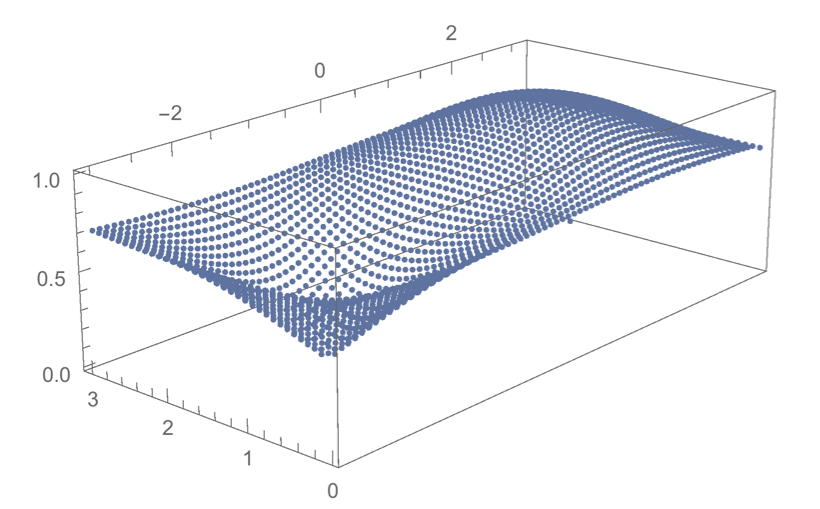
\includegraphics[width=\linewidth]{hypercomp/AmbisonicFieldAngle.png}
  \caption{Calculating the cylindrical projection of single ambisonic panned
    source in the Wolfram Mathematica software package}
  \label{fig:hypercomp-mathematica}
\end{figure}

\begin{figure}[]
 
\includegraphics[width=3.5cm]{hypercomp/left_x72.png}
 
\includegraphics[width=3.5cm]{hypercomp/above_x72.png}
 
\includegraphics[width=3.5cm]{hypercomp/front_x72.png}
 % 
\includegraphics[width=3.5cm]{hypercomp/right_x72.png}
 % 
\includegraphics[width=3.5cm]{hypercomp/below_x72.png}
 % 
\includegraphics[width=3.5cm]{hypercomp/rear_x72.png}
  \caption{Influence maps of 3 first-order spherical harmonics: left, top, and
    front. Pure white is $-0$~dBFS black is -inf~dBFS. Cylindrical projection.}
  \label{fig:hypercomp-inf-maps}
\end{figure}

\paragraph{Results:}If the input to the level detector is encoded as
an ambisonic plane wave, this level detector does yield accurate
results.  In the more common case, when our ambisonic input material
contains multiple sources that are each ambisonically panned to
different positions, this interpolation technique does not accurately
calculate the RMS at any angle. In simple cases, where we can be sure
our input material is appropriate, the technique described here might
be useful, but in most cases, a different approach will be more
effective.

\begin{figure}[h]
%  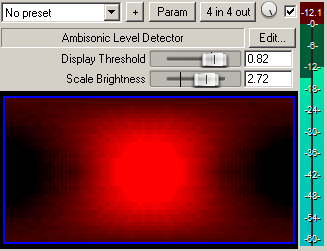
\includegraphics{hypercomp/LevelDetect_front.png}
  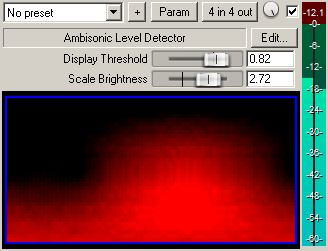
\includegraphics{hypercomp/LevelDetect_45_down.png}
  \caption{The Hypercompressor visualizer written for the efficient
    ambisonic level detector. The surround sphere is projected to a
    cylinder and unwrapped on the flat surface. In this image, a
    monophonic source is panned slightly down and to the right
    ($-45\degree$ azimuth, $-45\degree$ elevation).}
  \label{fig:hypercomp-inf-map-angle}
\end{figure}

\subsection{Ambisonic Gain Control Module}
\label{sec:ambis-gain-contr}
The spherical harmonics defined in equation~\ref{eq:ambisonics} form a
set of orthogonal basis functions. If we define a sequence for our
spherical harmonics and spherical harmonic expansion coefficients, we
can treat the expansion coefficients as vectors and perform matrix
operations on them that rotate, warp, and re-orient our
three-dimensional surround sound image.\cite{Pomberger2011} The
ability to mathematically warp and manipulate our surround sound image
makes ambisonics the perfect choice for implementing a surround sound
compressor.

\paragraph{The Focus Transform} One transform that lets us attenuate a
region of the surround sound sphere is the \textit{focus} transform
distributed as part of the open source Ambisonic Toolkit
(ATK)\sidenote{\url{http://www.ambisonictoolkit.net/}} This transform
is intended to focus on transform is intended to focus on the 
\cite{Anderson2009}
\begin{fullwidth}
\[ \left( \begin{array}{cccc}
\frac{1}{1 + \sin|w|} & 
\frac{1}{\sqrt{2}} \frac{\sin(w)}{1 + \sin|w|}  & 
0 &
0 \\
\sqrt{2}\frac{sin(w)}{1 + \sin|w|} & % LG1
\frac{1}{1 + \sin|w|} &                    % LG0
0 & 
0 \\
0 & 
0 &
\frac{\cos(w)}{1 + \sin(w)} &
0 \\
0 &
0 &
0 &
\frac{\cos(w)}{1 + \sin|w|} 
\end{array} \right)
\]
\end{fullwidth}
%%% Local Variables:
%%% mode: latex
%%% TeX-master: "CharlesHolbrow_MAS_Thesis"
%%% End:


\backmatter
\chapter*{Acknowledgements}
\label{ch:acknowledgements}

\begin{fullwidth}
Thanks to Tod Machover, for your continuous support and encouragement,
for sharing your process, and for help and support integrating \thesis
into \textit{Of Experience}.

Thanks to James Andy Moorer and Joe Paradiso for support, guidance and
mentorship.\TODO{verify spelling}

Thanks to professor Alex Case for the most inspiring my love for
music, audio engineering, and illuminating the magical subtleties of
dynamic range compression.

Thanks to Wonshik Choi and Niyom Lue for your infinite patience,
guidance, and for welcoming me to MIT in 2008. Only you could have
taught a music major to enjoy linux, DSP, and spectroscopy.

Thanks to Shawn Drost for directly and indirectly giving me confidence
as a software developer.

Thanks to my UMass Lowell Piano teachers for taking chance with me,
and putting up with me for four years. Anthony Mele, Elizabeth
Skavish, Bonnie Anderson, and Thomas Stumpf - You believed in me
before I did. I'm probably the only student ever who was lucky enough
to study with all four of you. :P

Thanks to Gene Atwood for being considerate of everyone, and showing
me how important that is -- And for screaming in to a microphone when
I needed some screams.

Thanks to Ben Bloomberg for being my peer and my mentor at the same
time. Thanks for bringing me into the Opera group in 2008 and bringing
me back in 2014. Thanks to Bryn Bliska, for proposing polytempic
modulation, and sharing letting me work out the maths. Thanks to
Rebecca Kleinberger and Akito Van Troyer for your unending support and
encouragement. 

Thanks to Helen Corless for being amazing supportive even when I am in
the absolute pits of grad student existence. Thank you for always
reminding me what music is really about, and for challenging me like
no one else can.

Thanks to my grandparents for leading by example, and teaching
kindness and dedication, and for endless support in education.

Thanks to Hilary, Giles, and Felicity for always inspiring me with
kindness, honesty, and wisdom. 

And thanks to my parents, Gwen and Mark for forcing me to get an
education before I was wise enough to know I wanted one. Thank you for
all your love and support in everything ever I have ever done.
\end{fullwidth}
%%% Local Variables:
%%% mode: latex
%%% TeX-master: t
%%% End:


\bibliography{library}
\bibliographystyle{plainnat}

\end{document}


%%% Local Variables:
%%% mode: latex
%%% TeX-master: t
%%% End:
